\documentclass{article}
\usepackage[paperwidth=22cm, paperheight=13cm, margin=0.5cm]{geometry}
\pagestyle{empty}
\usepackage{tikz}
\usetikzlibrary{arrows.meta, fit, backgrounds, calc}
\usepackage{xcolor}

% ── Palette ───────────────────────────────────────────────────────────────────
\definecolor{cInput}{HTML}{EDE8DC}  \definecolor{bInput}{HTML}{8B7355}
\definecolor{cChan} {HTML}{FDEBD0}  \definecolor{bChan} {HTML}{CA6F1E}
\definecolor{cProc} {HTML}{EAF3FB}  \definecolor{bProc} {HTML}{2980B9}
\definecolor{cMask} {HTML}{D5F5E3}  \definecolor{bMask} {HTML}{1A8048}
\definecolor{cAn}   {HTML}{D6EEF8}  \definecolor{bAn}   {HTML}{117A8B}
\definecolor{cOut}  {HTML}{D4EDDA}  \definecolor{bOut}  {HTML}{1D7A38}
\definecolor{bgSeg} {HTML}{EAEAF5}  \definecolor{bdSeg} {HTML}{8888C0}
\definecolor{bgAn}  {HTML}{DDF0F7}  \definecolor{bdAn}  {HTML}{17A2B8}
\definecolor{bgOut} {HTML}{E0F2E5}  \definecolor{bdOut} {HTML}{28A745}

% ── Styles ────────────────────────────────────────────────────────────────────
\tikzset{
  box/.style={draw, rounded corners=5pt, align=center, font=\small,
              minimum height=1.15cm, text width=2.15cm,
              inner sep=5pt, line width=0.85pt},
  inputbox/.style={box, fill=cInput, draw=bInput},
  chanbox/.style ={box, fill=cChan,  draw=bChan},
  procbox/.style ={box, fill=cProc,  draw=bProc},
  maskbox/.style ={box, fill=cMask,  draw=bMask},
  anbox/.style   ={box, fill=cAn,    draw=bAn, text width=2.4cm},
  outbox/.style  ={box, fill=cOut,   draw=bOut},
  arr/.style={-{Stealth[length=5pt,width=4pt]}, draw=gray!60, line width=0.9pt},
  seclbl/.style={font=\footnotesize\itshape, text=gray!65!black},
}

\newcommand{\sub}[1]{{\fontsize{7}{9}\selectfont #1}}

\begin{document}
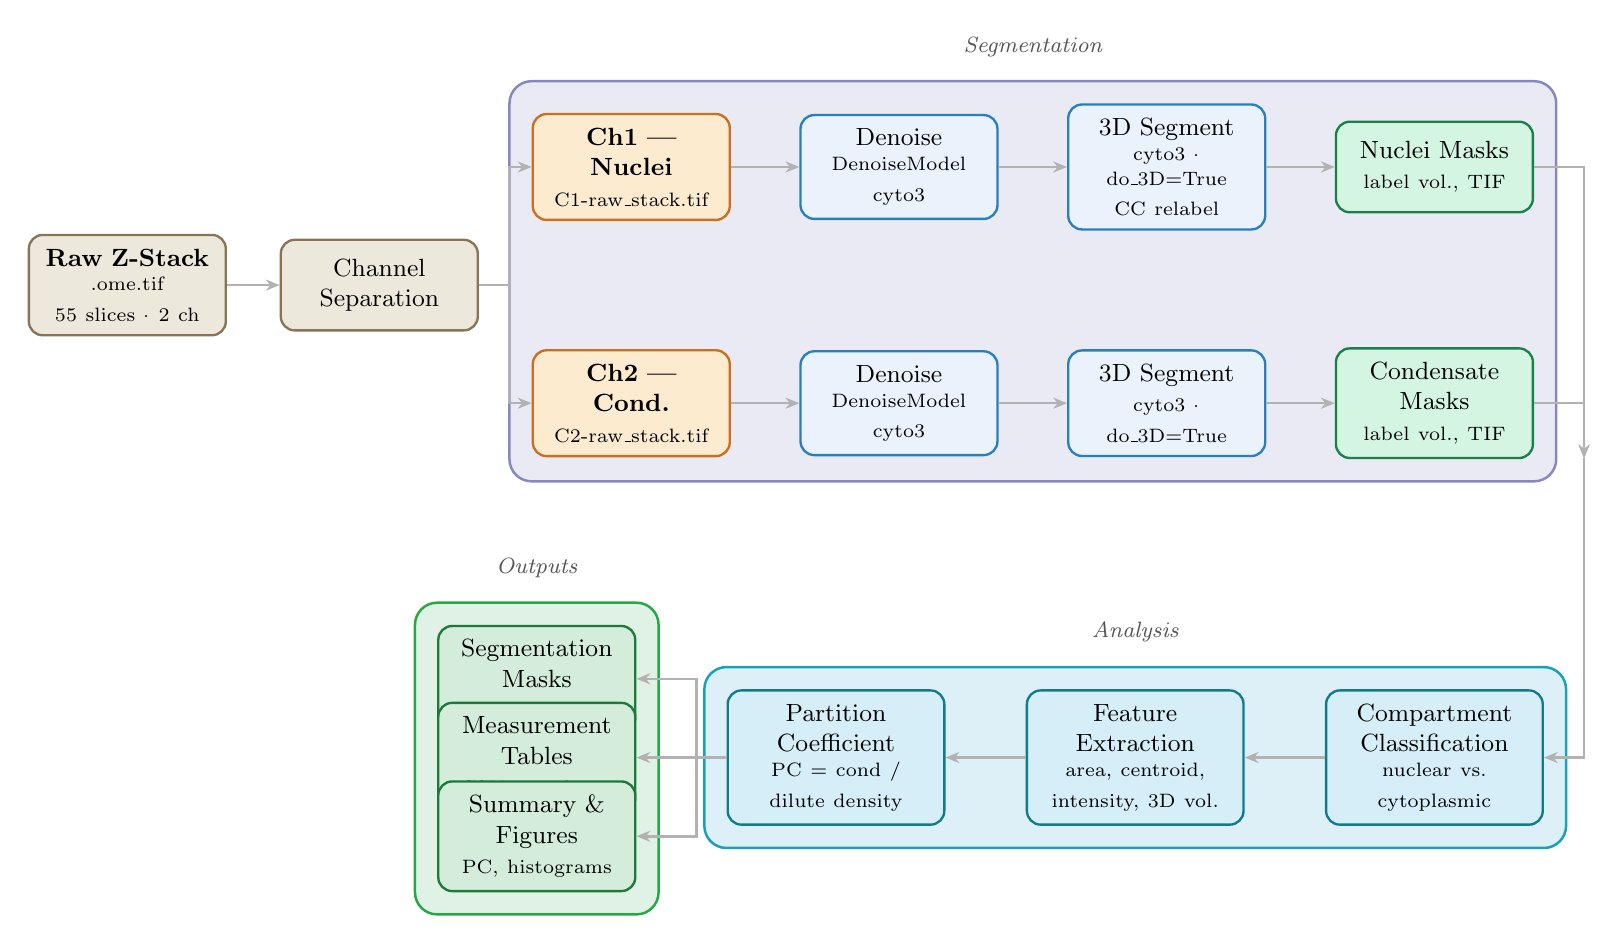
\begin{tikzpicture}

% ── Y levels ──────────────────────────────────────────────────────────────────
% Row 1 (top, left → right)
\def\ytop{4.5}
\def\ymid{3.0}
\def\ybot{1.5}
% Row 2 (bottom, right → left)
\def\yrow{-3.0}
\def\ytopo{-2.0}
\def\yboto{-4.0}

% ── Row 1 Nodes ───────────────────────────────────────────────────────────────

\node[inputbox] (raw) at (0, \ymid)
  {\textbf{Raw Z-Stack}\\\sub{.ome.tif\\55 slices · 2 ch}};

\node[inputbox] (chsep) at (3.2, \ymid)
  {Channel\\Separation};

\node[chanbox] (ch1) at (6.4, \ytop)
  {\textbf{Ch1 — Nuclei}\\\sub{C1-raw\_stack.tif}};

\node[chanbox] (ch2) at (6.4, \ybot)
  {\textbf{Ch2 — Cond.}\\\sub{C2-raw\_stack.tif}};

\node[procbox] (dn1) at (9.8, \ytop)
  {Denoise\\\sub{DenoiseModel\\cyto3}};

\node[procbox] (dn2) at (9.8, \ybot)
  {Denoise\\\sub{DenoiseModel\\cyto3}};

\node[procbox] (seg1) at (13.2, \ytop)
  {3D Segment\\\sub{cyto3 · do\_3D=True\\CC relabel}};

\node[procbox] (seg2) at (13.2, \ybot)
  {3D Segment\\\sub{cyto3 · do\_3D=True}};

\node[maskbox] (mask1) at (16.6, \ytop)
  {Nuclei Masks\\\sub{label vol., TIF}};

\node[maskbox] (mask2) at (16.6, \ybot)
  {Condensate\\Masks\\\sub{label vol., TIF}};

% ── Row 2 Nodes (right → left) ────────────────────────────────────────────────

\node[anbox] (cc) at (16.6, \yrow)
  {Compartment\\Classification\\\sub{nuclear vs.\\cytoplasmic}};

\node[anbox] (fe) at (12.8, \yrow)
  {Feature\\Extraction\\\sub{area, centroid,\\intensity, 3D vol.}};

\node[anbox] (pc) at (9.0, \yrow)
  {Partition\\Coefficient\\\sub{PC = cond /\\dilute density}};

\node[outbox] (out1) at (5.2, \ytopo)
  {Segmentation\\Masks\\\sub{TIF stacks}};

\node[outbox] (out2) at (5.2, \yrow)
  {Measurement\\Tables\\\sub{CSV per object}};

\node[outbox] (out3) at (5.2, \yboto)
  {Summary \&\\Figures\\\sub{PC, histograms}};

% ── Arrows ────────────────────────────────────────────────────────────────────

% Row 1: input chain
\draw[arr] (raw) -- (chsep);
\draw[arr] (chsep.east) -- ++(0.38,0) |- (ch1.west);
\draw[arr] (chsep.east) -- ++(0.38,0) |- (ch2.west);

% Nuclei track
\draw[arr] (ch1)  -- (dn1);
\draw[arr] (dn1)  -- (seg1);
\draw[arr] (seg1) -- (mask1);

% Condensate track
\draw[arr] (ch2)  -- (dn2);
\draw[arr] (dn2)  -- (seg2);
\draw[arr] (seg2) -- (mask2);

% Row 1 → Row 2: both masks merge at right-side junction, then U-turn down to CC
\draw[arr] (mask1.east) -| (18.5, 0.8);
\draw[arr] (mask2.east) -| (18.5, 0.8);
\draw[arr] (18.5, 0.8) -- (18.5, \yrow) -- (cc.east);

% Row 2: analysis chain (right → left)
\draw[arr] (cc.west) -- (fe.east);
\draw[arr] (fe.west) -- (pc.east);

% Fan out to outputs
\draw[arr] (pc.west) -- ++(-0.38,0) |- (out1.east);
\draw[arr] (pc.west) -- ++(-0.38,0) |- (out2.east);
\draw[arr] (pc.west) -- ++(-0.38,0) |- (out3.east);

% ── Section backgrounds ───────────────────────────────────────────────────────
\begin{scope}[on background layer]
  \node[fill=bgSeg, draw=bdSeg, rounded corners=8pt,
        fit=(ch1)(ch2)(dn1)(dn2)(seg1)(seg2)(mask1)(mask2),
        inner sep=8pt, line width=0.9pt] (segbg) {};
  \node[fill=bgAn, draw=bdAn, rounded corners=8pt,
        fit=(cc)(fe)(pc),
        inner sep=8pt, line width=0.9pt] (anbg) {};
  \node[fill=bgOut, draw=bdOut, rounded corners=8pt,
        fit=(out1)(out2)(out3),
        inner sep=8pt, line width=0.9pt] (outbg) {};
\end{scope}

% ── Section labels ────────────────────────────────────────────────────────────
\node[seclbl] at ([yshift=5pt] segbg.north) [above] {\textit{Segmentation}};
\node[seclbl] at ([yshift=5pt] anbg.north)  [above] {\textit{Analysis}};
\node[seclbl] at ([yshift=5pt] outbg.north) [above] {\textit{Outputs}};

\end{tikzpicture}
\end{document}